 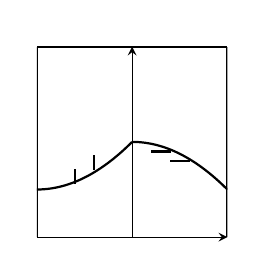
\begin{tikzpicture}
        \begin{axis}[
            axis lines = middle,
            xlabel = $ $,
            ylabel = $ $,
            xmin = -0.5, xmax = 0.5,
            ymin = 0, ymax = 1,
            xtick = {0},
            ytick = {0},
            x label style={at={(axis description cs:1,0)},anchor=west},
            y label style={at={(axis description cs:0,1)},anchor=south},
            extra tick style={grid=major},
            width=4cm, height=4cm,
            samples=100,
            domain=-0.5:0.5,
        ]
                \addplot[domain=-0.5:0, samples=100, thick] {0.25+(x+0.5)^2};
                \draw [thick](-0.5,0) -- (-0.5,1);
                \draw [thick](0.5,0) -- (0.5,1);
                \draw [thick](0.5,1) -- (-0.5,1);
                \addplot[domain=0.1:0.2, samples=100, thick] {0.45};
                \addplot[domain=0.2:0.3, samples=100, thick] {0.40};
                \draw [thick](-0.2,0.35) -- (-0.2,0.43);
                \draw [thick](-0.3,0.28) -- (-0.3,0.36);
        \addplot[domain=0:0.5, samples=100, thick] {0.5-x^2};
        \end{axis}
    \end{tikzpicture}
    
